\chapter{Market Analysis}
\label{sec:market}

In order to evaluate AndroMEDA effectiveness in identifying malware, it's important to evaluate the ability to identify malware without it. As previously discussed in \ref{sec:permissions}, Permissions are the single security measure that defends an Android user from malicious software. We hope to show a fundamental disconnect between Permissions and UAA, as conclusive evidence that Permissions should not be the sole security system on Android. In order to study this, we must examine the how Permissions reflect app behavior, and if known malware can be identified with Permissions alone.


\begin{table*}[t]
\begin{small}
\begin{tabular}{l|lll}
Scan Timestamp & Number of Apps &  \\
\hline

\textit{fill this in} & I should fill this in  \\

\end{tabular}
\end{small}
%\vspace{-0.2in}
\caption{Statistics from \temp{AndroidMarketDB}}
\label{tab:marketstats}
%\vspace{-0.1in}
\end{table*}


\begin{table*}[t]
\begin{small}
\begin{tabular}{r|l}
Metadata & Description \\
\hline

\textit{App Name} & The name of the app, e.g. Google Maps  \\
\textit{App Developer} & The name of the developer, e.g. Google  \\
\textit{Android Version} & The lowest compatible Android version  \\
\textit{Number of Installs} &  The total number of installs. Given as a range. \\
\textit{Description} &  A long (3000 word max) description of the app. \\
\textit{Reviews} &  The user reviews of the app. \\
\textit{Overall Rating} &  The overall rating of the app, from 1 to 5. A user does not need to write a review to leave a rating. \\
\textit{Requested Permissions} &  The list of all the permissions the app requests. \\

\end{tabular}
\end{small}
%\vspace{-0.2in}
\caption{Metadata from \temp{AndroidMarketDB}}
\label{tab:marketmetadata}
%\vspace{-0.1in}
\end{table*}





\section{Market Dataset}
To do a broad scale study of Android permissions, we introduce a novel dataset: \temp{AndroidMarketDB}. \temp{AndroidMarketDB} contains metadata from \temp{80\%} of all known Android Apps in the GPStore, see Table \ref{tab:marketstats}. This metadata, described in \ref{tab:marketmetadata}, is rich in contextual information about an app. For a period of 1 month in May-June 2012, the GPStore was scanned twice a day. This dataset provides detailed metadata for all areas of the Android market, not just the top percent. Despite the large amount of metadata available, we will focus on the Permissions, leaving most other fields for Future Work\ref{sec:futurework}.

% Should have some figures demonstrating how big this dataset is.

\section{Global Permission Analysis}
We first look at the global trends of Permissions in the GPStore. Ideally, we find that access to sensitive PII, and dangerous operations, only is requested by a handful of apps that truly need them. This both increases the user's ability to understand how an app behaves, increases the user's trust in the Permission system, and demonstrates a strong connection between Permission Fingerprint and User-App Agreement. Ultimately, however, we expect to find a system that falls short of these goals.

\begin{figure}[h]
\begin{center}
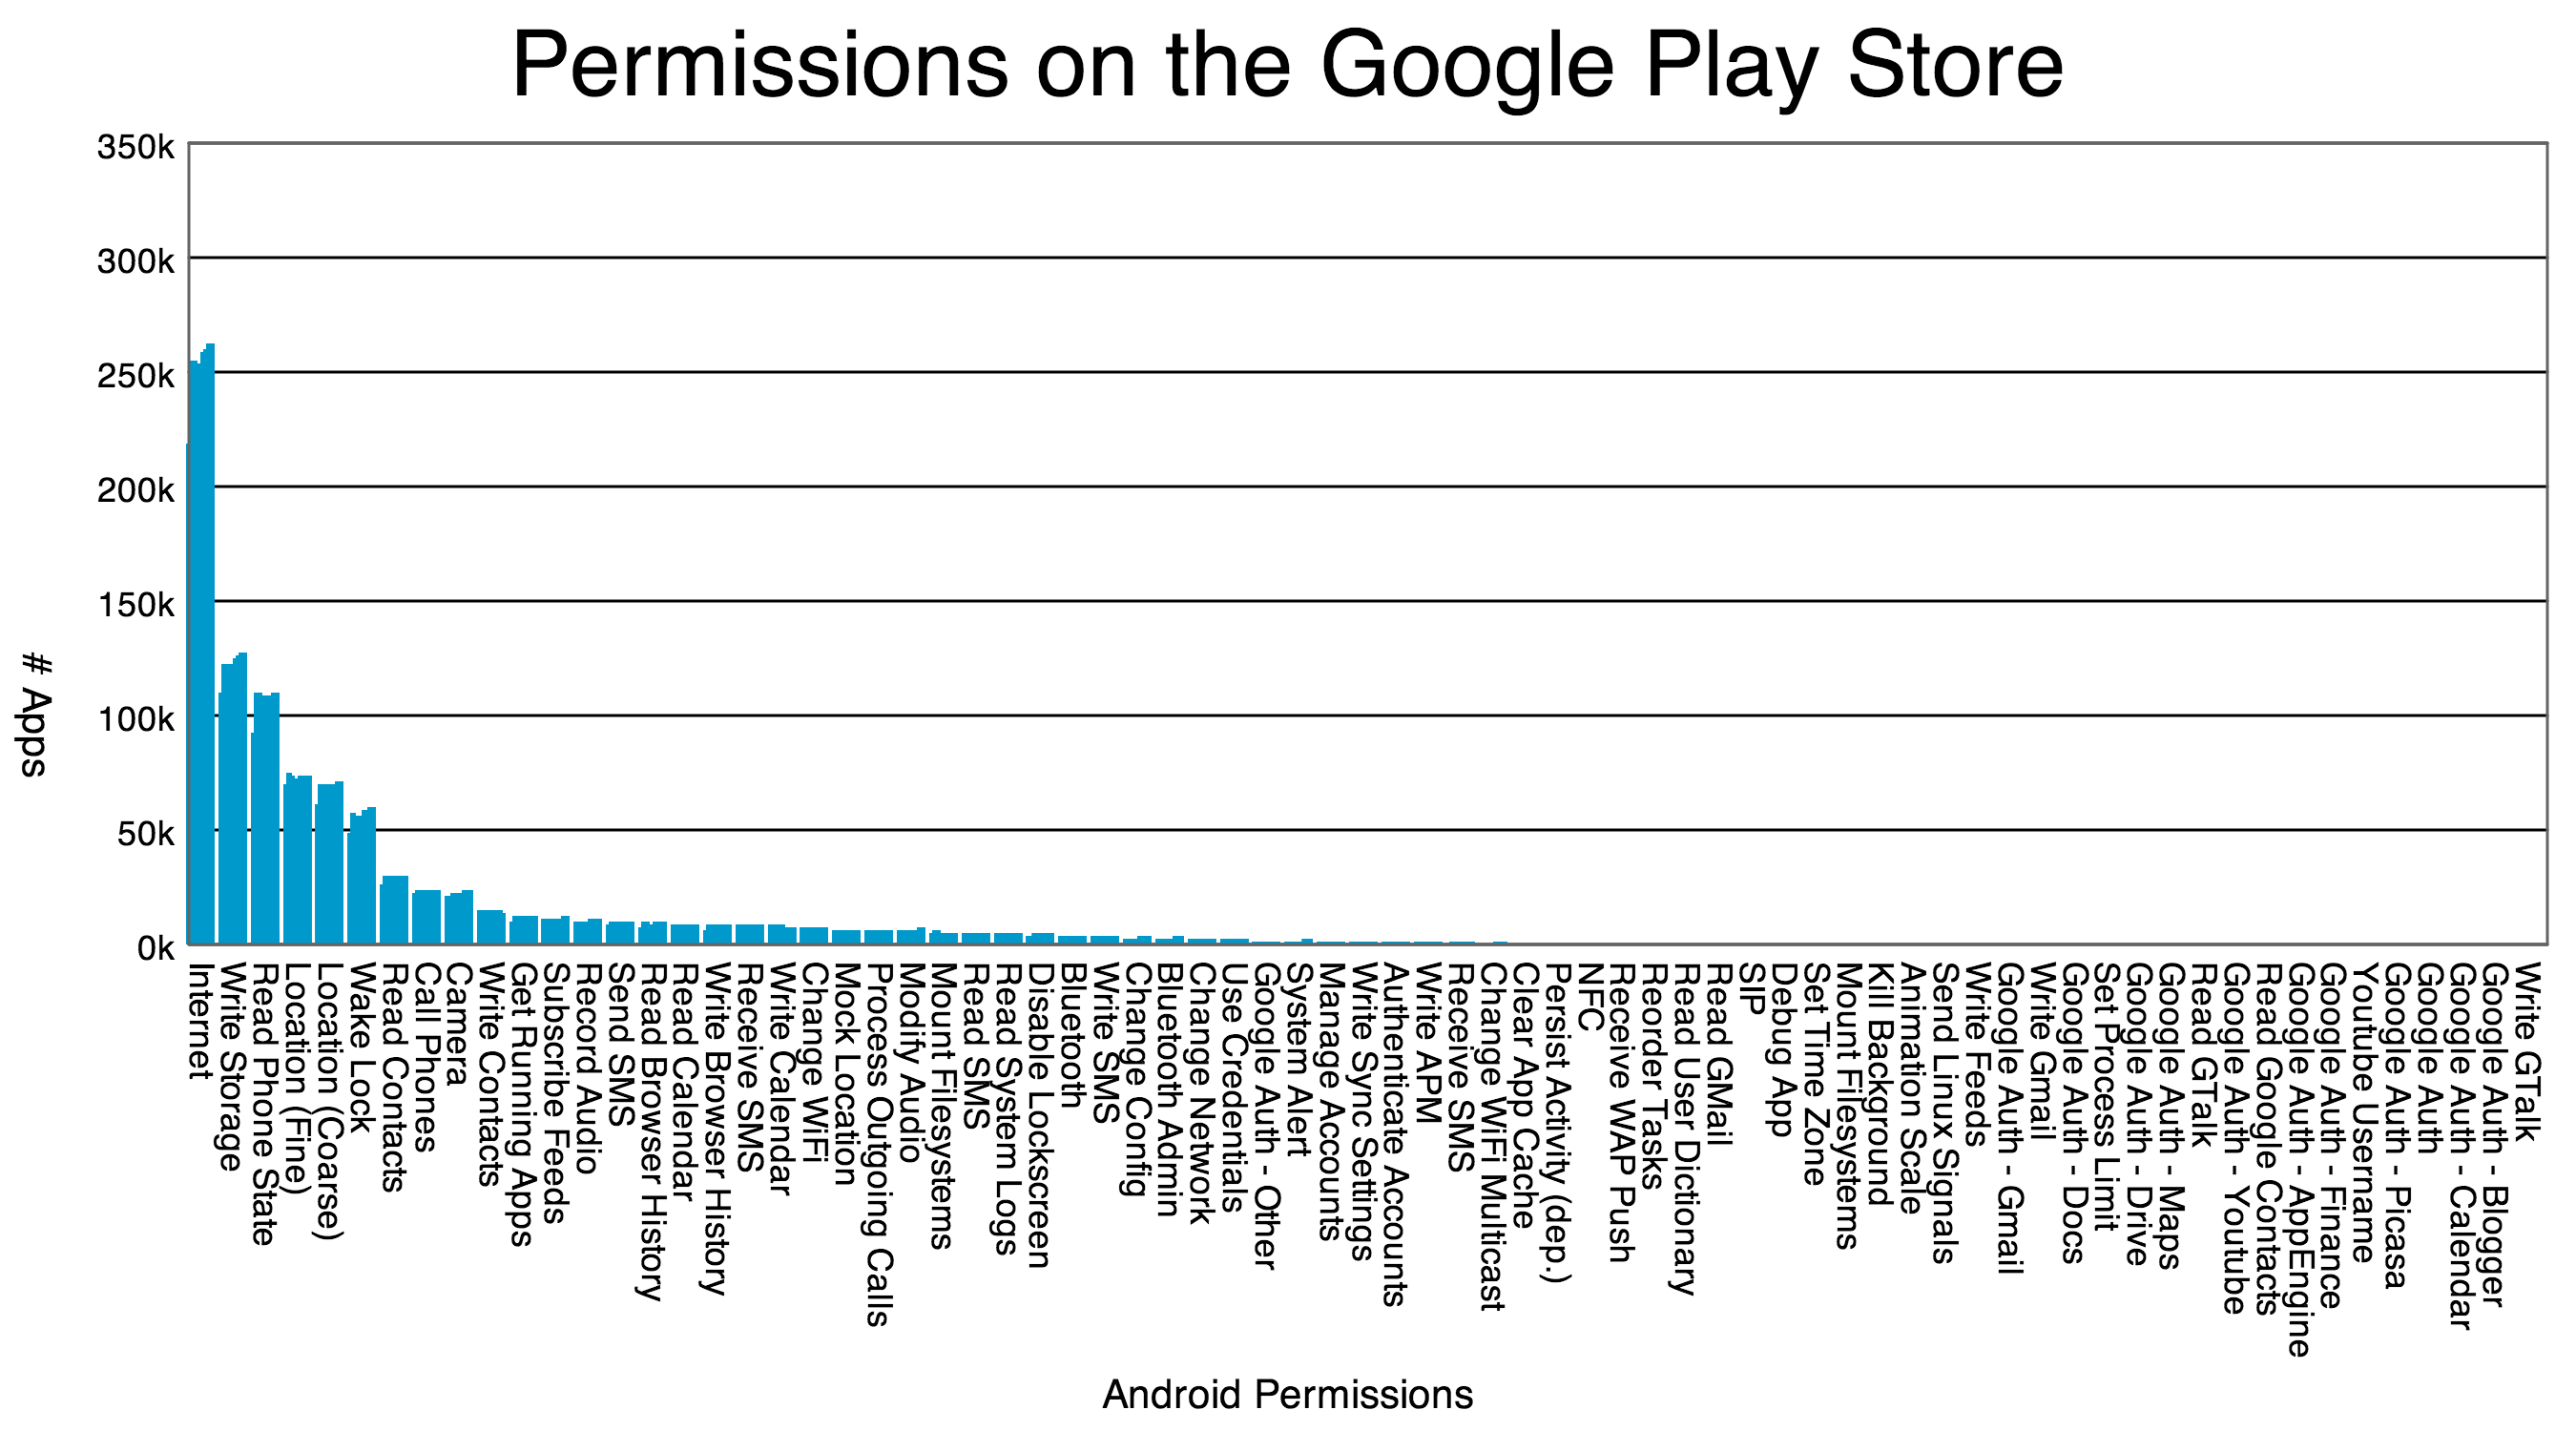
\includegraphics[width=1.0\columnwidth]{figs/AllPermissions}
\caption{Permissions, sorted by how many apps request them in the entire GPStore dataset}
\label{fig:allpermissions}
\end{center}
\end{figure}

\begin{figure}[h]
\begin{center}
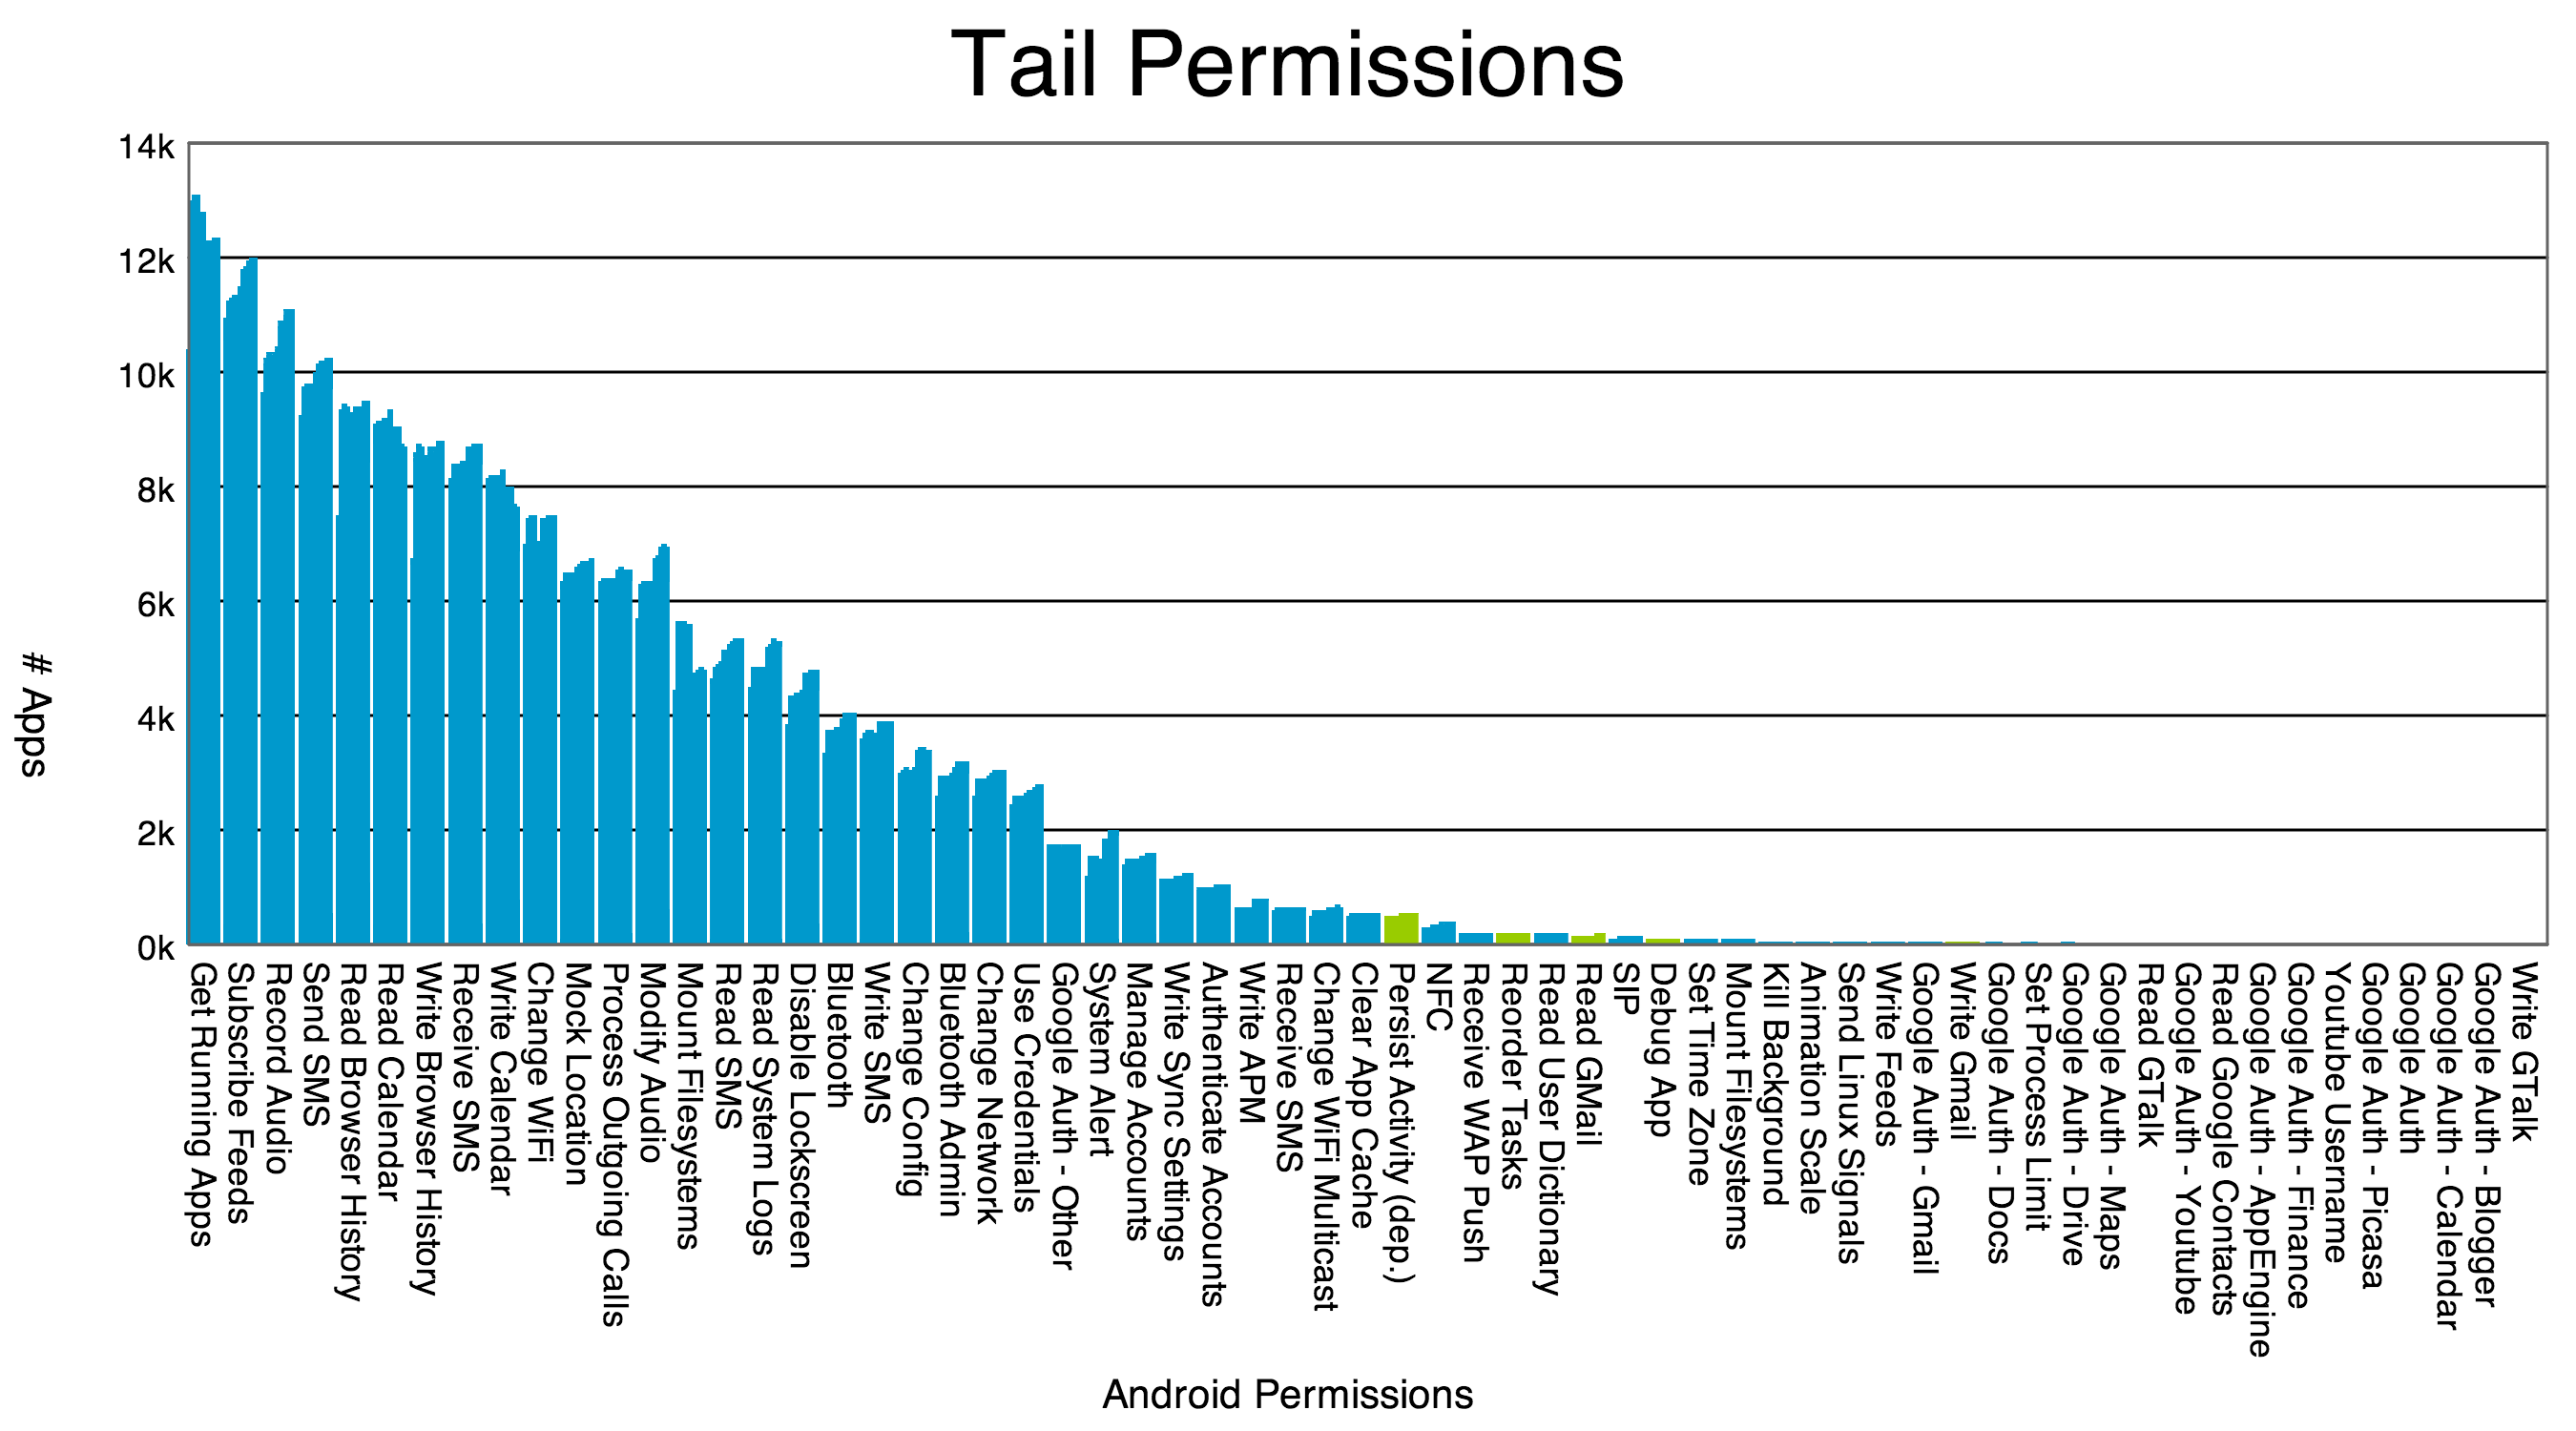
\includegraphics[width=1.0\columnwidth]{figs/AllPermissions_Tail}
\caption{Less commonly used permissions in the GPStore}
\label{fig:tailpermissions}
\end{center}
\end{figure}

Figure \ref{fig:allpermissions} shows all major permissions in the GPStore, sorted by frequency of use. This graph highlights several things: First off, \textit{INTERNET} is a dominant permission, with well over half of the GPStore apps requesting it. The next 5 permissions, \textit{Write to Storage}, \textit{Reading Phone Info}, \textit{Location Info} and \textit{Wake Lock}, all have over 50,000 apps that request them. A steep drop is seen for \textit{Read Contacts}, \textit{Call Phones}, and \textit{Camera}, with around 25,000 apps each. Of these top 9, 3 provide access to semi-personal information: \textit{Reading Phone Info} and the \textit{Location Info} permissions. It's only when we get to the lower 3 do we get access to personal information. 

Figure \ref{fig:tailpermissions} examines the tail permissions in the GPStore. This section contains the bulk of permissions related to PII, with \textit{Record Audio}, \textit{Read Calendar}, \textit{Read SMS}, and so on. It additionally contains many sensitive operations, like \textit{Send SMS} and \textit{System Alert} - which allows apps to draw windows over other apps. These permissions, while being a relatively small portion of the GPStore, still occupy a substantial portion. Indeed, with every dangerous permission, many legitimate use cases can be established, see Figure \ref{tab:permissionsanduses} for examples.

\begin{table*}[h]
\begin{small}
\begin{tabular}{p{3cm}|p{12.5cm}}
Permission & Use Case \\
\hline

\textit{Location (Fine)} & This one has a wide variety of uses, from location-specific news apps and games, to social networks. It's also used by ad networks included in many apps.  \\
\textit{Location (Coarse)} & This one follows the same trends as \textit{Location (Fine)}, but is skewed towards ad networks.  \\
\textit{Read Contacts} & Any access to the address book at all require this, so communication apps, social networks, or many apps that involve sharing with friends will use this.  \\
\textit{Call Phones} & This one is oddly popular. Many customization apps, especially those that seek to replace stock Android apps, will use this, especially if they are replacing address book or home screen functionalities. Additionally, many communication apps will use this, for obvious reasons.  \\
\textit{Camera} & Any photography app or video camera app will make heavy use of this permission. This functionality is often present in other apps as well, e.g. taking a photo of the user for use as a profile photo  \\
\textit{Write Contacts} & This permission is often used with \textit{Read Contacts}. Many social networking sites and services wish to provide ``contact syncing'' abilities with Android device, which requires having write-access to the Contacts database.  \\
\textit{Record Audio} & Like \textit{Camera}, audio apps and communication apps make heavy use of this.  \\
\textit{Send SMS} & Many apps seek to replace the default SMS app, which would therefore require all of the SMS related permissions.  \\
\textit{System Alert} & This permission protects drawing on the screen, on top of other apps. Many apps are designed to be on the screen at all times, either replacing Android components, or complementing them.  \\

\end{tabular}
\end{small}
%\vspace{-0.2in}
\caption{Use cases for common Android Permissions}
\label{tab:permissionsanduses}
%\vspace{-0.1in}
\end{table*}

\subsection{Per Market Category}
Overall, we find many PII related permissions are requested a substantial number of times. A number of use cases exist, but it remains to be seen if the apps follow those use cases. To further examine this, we separate the apps in \temp{AndroidMarketDB} into the categories present on the GPStore, and rerun the analysis, seen in Figure \ref{fig:permissionspercategory}.

\begin{figure}[h]
\begin{center}
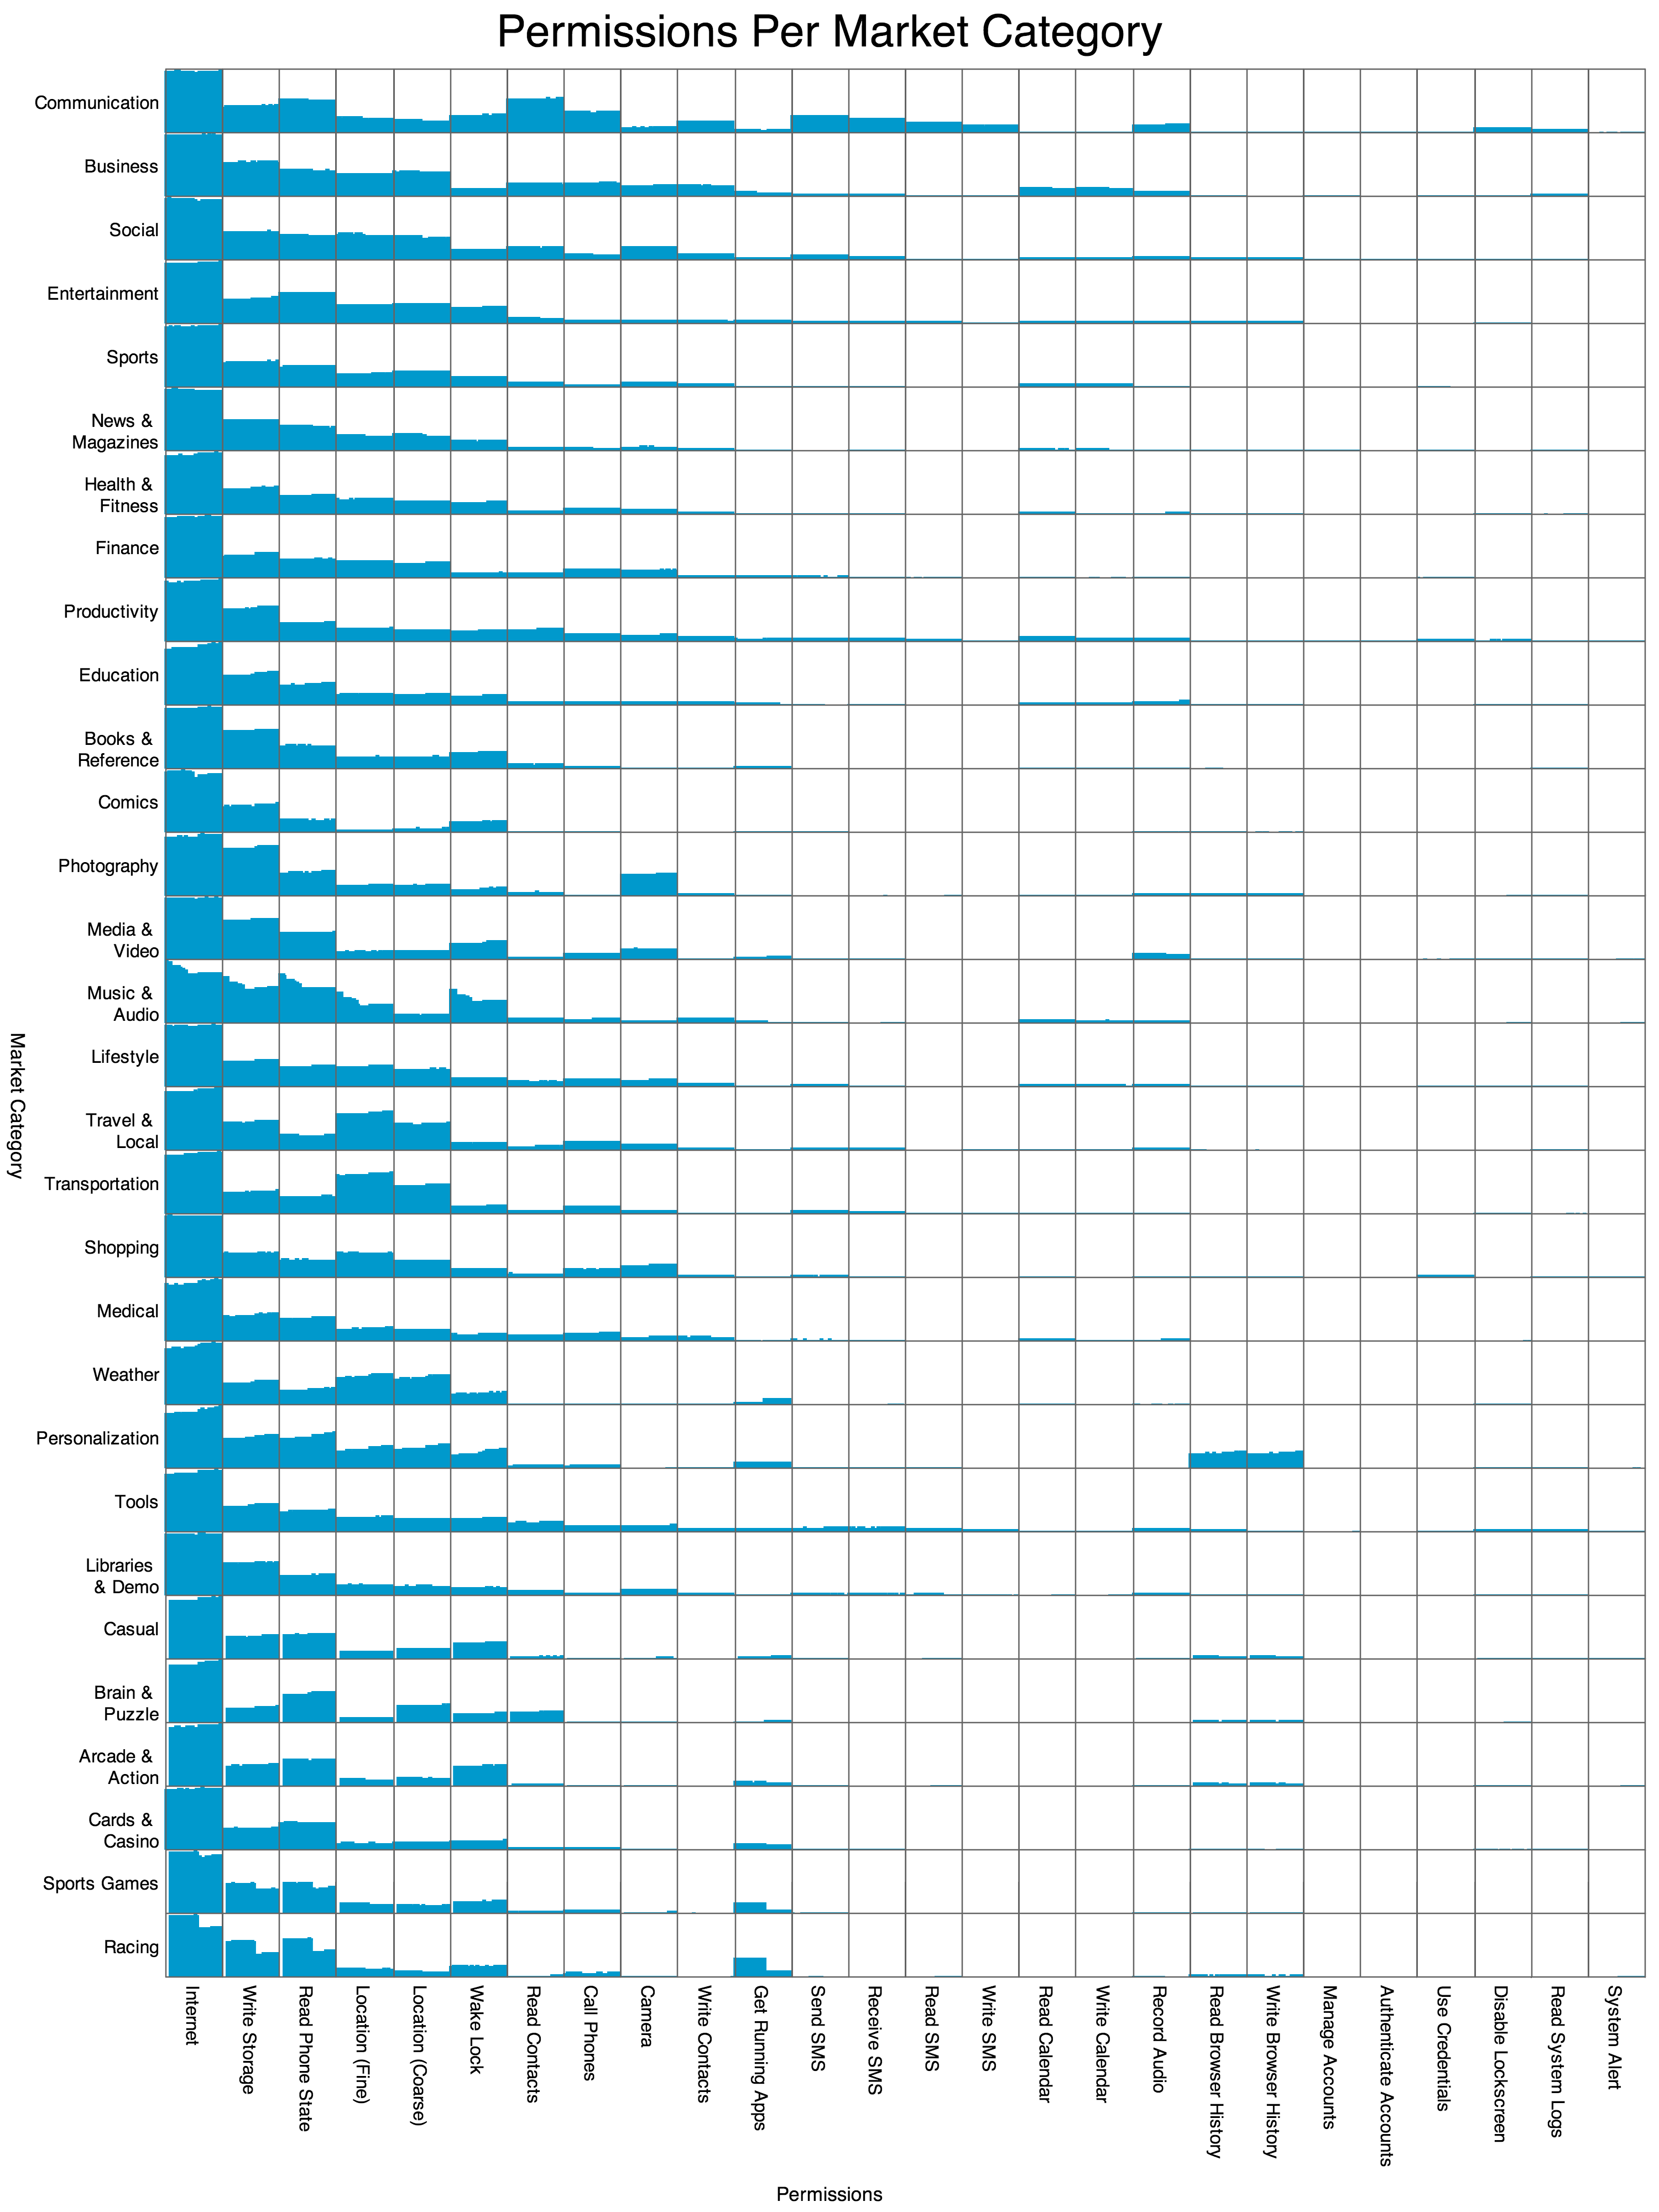
\includegraphics[width=1.0\columnwidth]{figs/PermissionsforMarketCategory}
\caption{Permissions used, as a fraction of total in that category}
\label{fig:permissionspercategory}
\end{center}
\end{figure}

Immediately, the use cases described in \ref{tab:permissionsanduses} become apparent. A large spike is seen in category \textit{Photography} and \textit{Media \& Video} for permission \textit{Camera}, similarly with \textit{Record Audio}, although it's less visible in \textit{Music \& Audio}. Location data is commonly used in \textit{Weather}, \textit{Transportation} and \textit{Travel}, another use case. \textit{Send SMS} is found predominantly in \textit{Communication} and \textit{Social}, another good sign. \textit{Wake Lock} was found heavily in games, music and media, and communication, but less so in other categories, as would be expected for it's use case.

Ultimately, however, some odd patterns can be observed. Despite \textit{Read Contacts} being popular for apps in \textit{Communication}, \textit{Business} and \textit{Social}, it's also found heavily in the \textit{Brain \& Puzzle} game category. A similar pattern is seen in \textit{Call Phones}; it's predominant category is \textit{Communication}, but it's found in significant amounts in \textit{Medical}, \textit{Shopping}, and \textit{Lifestyle}. We also find a spike in \textit{Get Running Apps} in games that does not appear to be present in other market categories. Perhaps the oddest observation was the extremely large spike of \textit{Read Browser History} and \textit{Write Browser History} found in the \textit{Personalization} category.

\temp{STUDY THESE THINGS AND REPORT WHAT THE HECK IS UP}

Overall, we've noted a number of times when patterns in permissions in the GPStore break our expectations of them - potentially violating them User-App Agreement. These could be detected simply from the Permission Fingerprint. We have shown a fairly strong correlation with major PII permissions and Android categories, but demonstrated many cases where they do not line up, both maliciously and with legitimate use cases.






\section{Malware Dataset}
Next, we compare a malware dataset with \temp{AndroidMarketDB}, in the hopes of finding them as outliers. Ideally, all malicious behavior would show up in the permission fingerprint of an app, so therefore it's unique set of capabilities would stand out in the Google Play Store. Demonstrating that expected behavior and Permission Fingerprint are correlated will be an important part of that. Ultimately, however, we expect this method to have it's shortcomings.


\begin{figure}[h]
\begin{center}
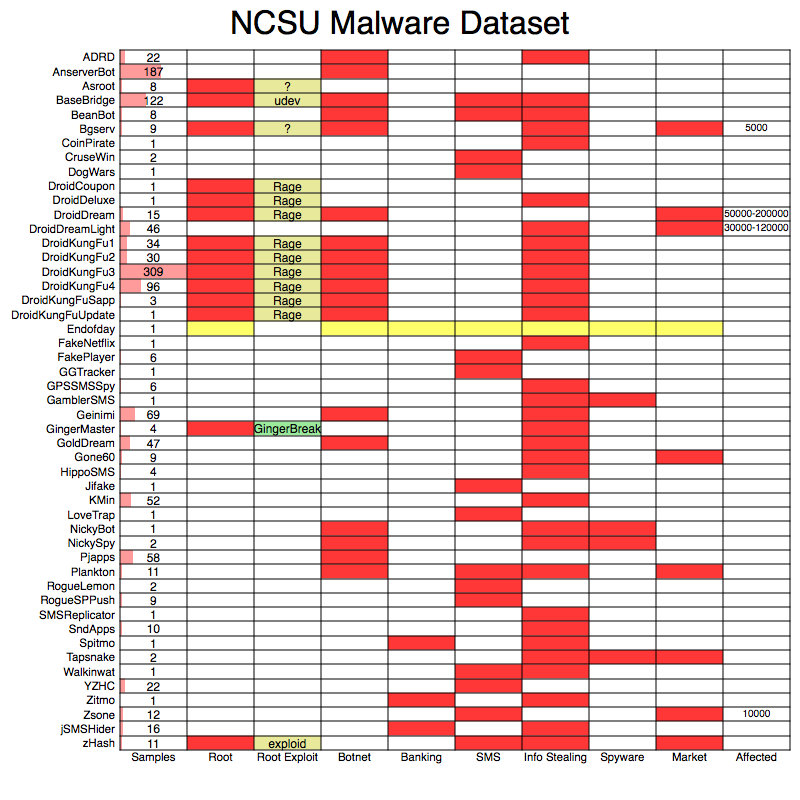
\includegraphics[width=0.85\columnwidth]{figs/NCSUMalwareDataset}
\caption{A summary of the malware families found in the Android Malware Genome Project}
\label{fig:malwaredboverview}
\end{center}
\end{figure}

\begin{table*}[h]
\begin{small}
\begin{tabular}{p{3cm}|p{12.5cm}}
Malware Class & Description \\
\hline

\textit{Root} & The malware uses a rootkit as a method of attack.    \\
\textit{Botnet} & The malware exhibits behavior associated with botnets, e.g. accepts remote commands.    \\
\textit{Banking} & The malware is designed specifically to intercept Banking messages.    \\
\textit{SMS} & The malware sends Premium SMS messages charged against the user.    \\
\textit{Info} &  The malware uploads personal information to a remote server, without notifying the user   \\
\textit{Spyware} & The malware remains on in the background, or has the capability of remotely monitoring the smartphone user.    \\
\textit{Market} &  The malware was spotted in the official Google Play Store   \\

\end{tabular}
\end{small}
%\vspace{-0.2in}
\caption{Malware Classes found in the Android Malware Genome Project}
\label{tab:malwaredbcategories}
%\vspace{-0.1in}
\end{table*}


\subsection{Android Malware Genome Project}
The dataset we use - the largest academic set of it's kind, is the Android Malware Genome Project\citep{zhou2012dissecting}, from NCSU. Containing almost 1300 samples from 52 families of actual Android malware, it provides the ideal test dataset for Android. We first classify each malware family by its capabilities, according to data aggregated by Spreitzenbarth\citep{spreitzenbarth2013} and Hackmageddon\citep{hackmageddon2011}, with the chart shown in Figure \ref{fig:malwaredboverview}, and the explanation of the classification of capabilities in Table \ref{tab:malwaredbcategories}.

Of the three classes of malware discussed in \ref{sec:malware}, we observe that very few of the malware families use only one attack vector - 6 families, all of which only used \textit{SMS} attacks, and 1, \textit{Pjapps} used none, only being a botnet. Clearly, Android Malware often uses multiple vectors. We also note that 33 of 52 - 63\% of all malware families upload personal information to a remote server. 

\begin{figure}[h]
\begin{center}
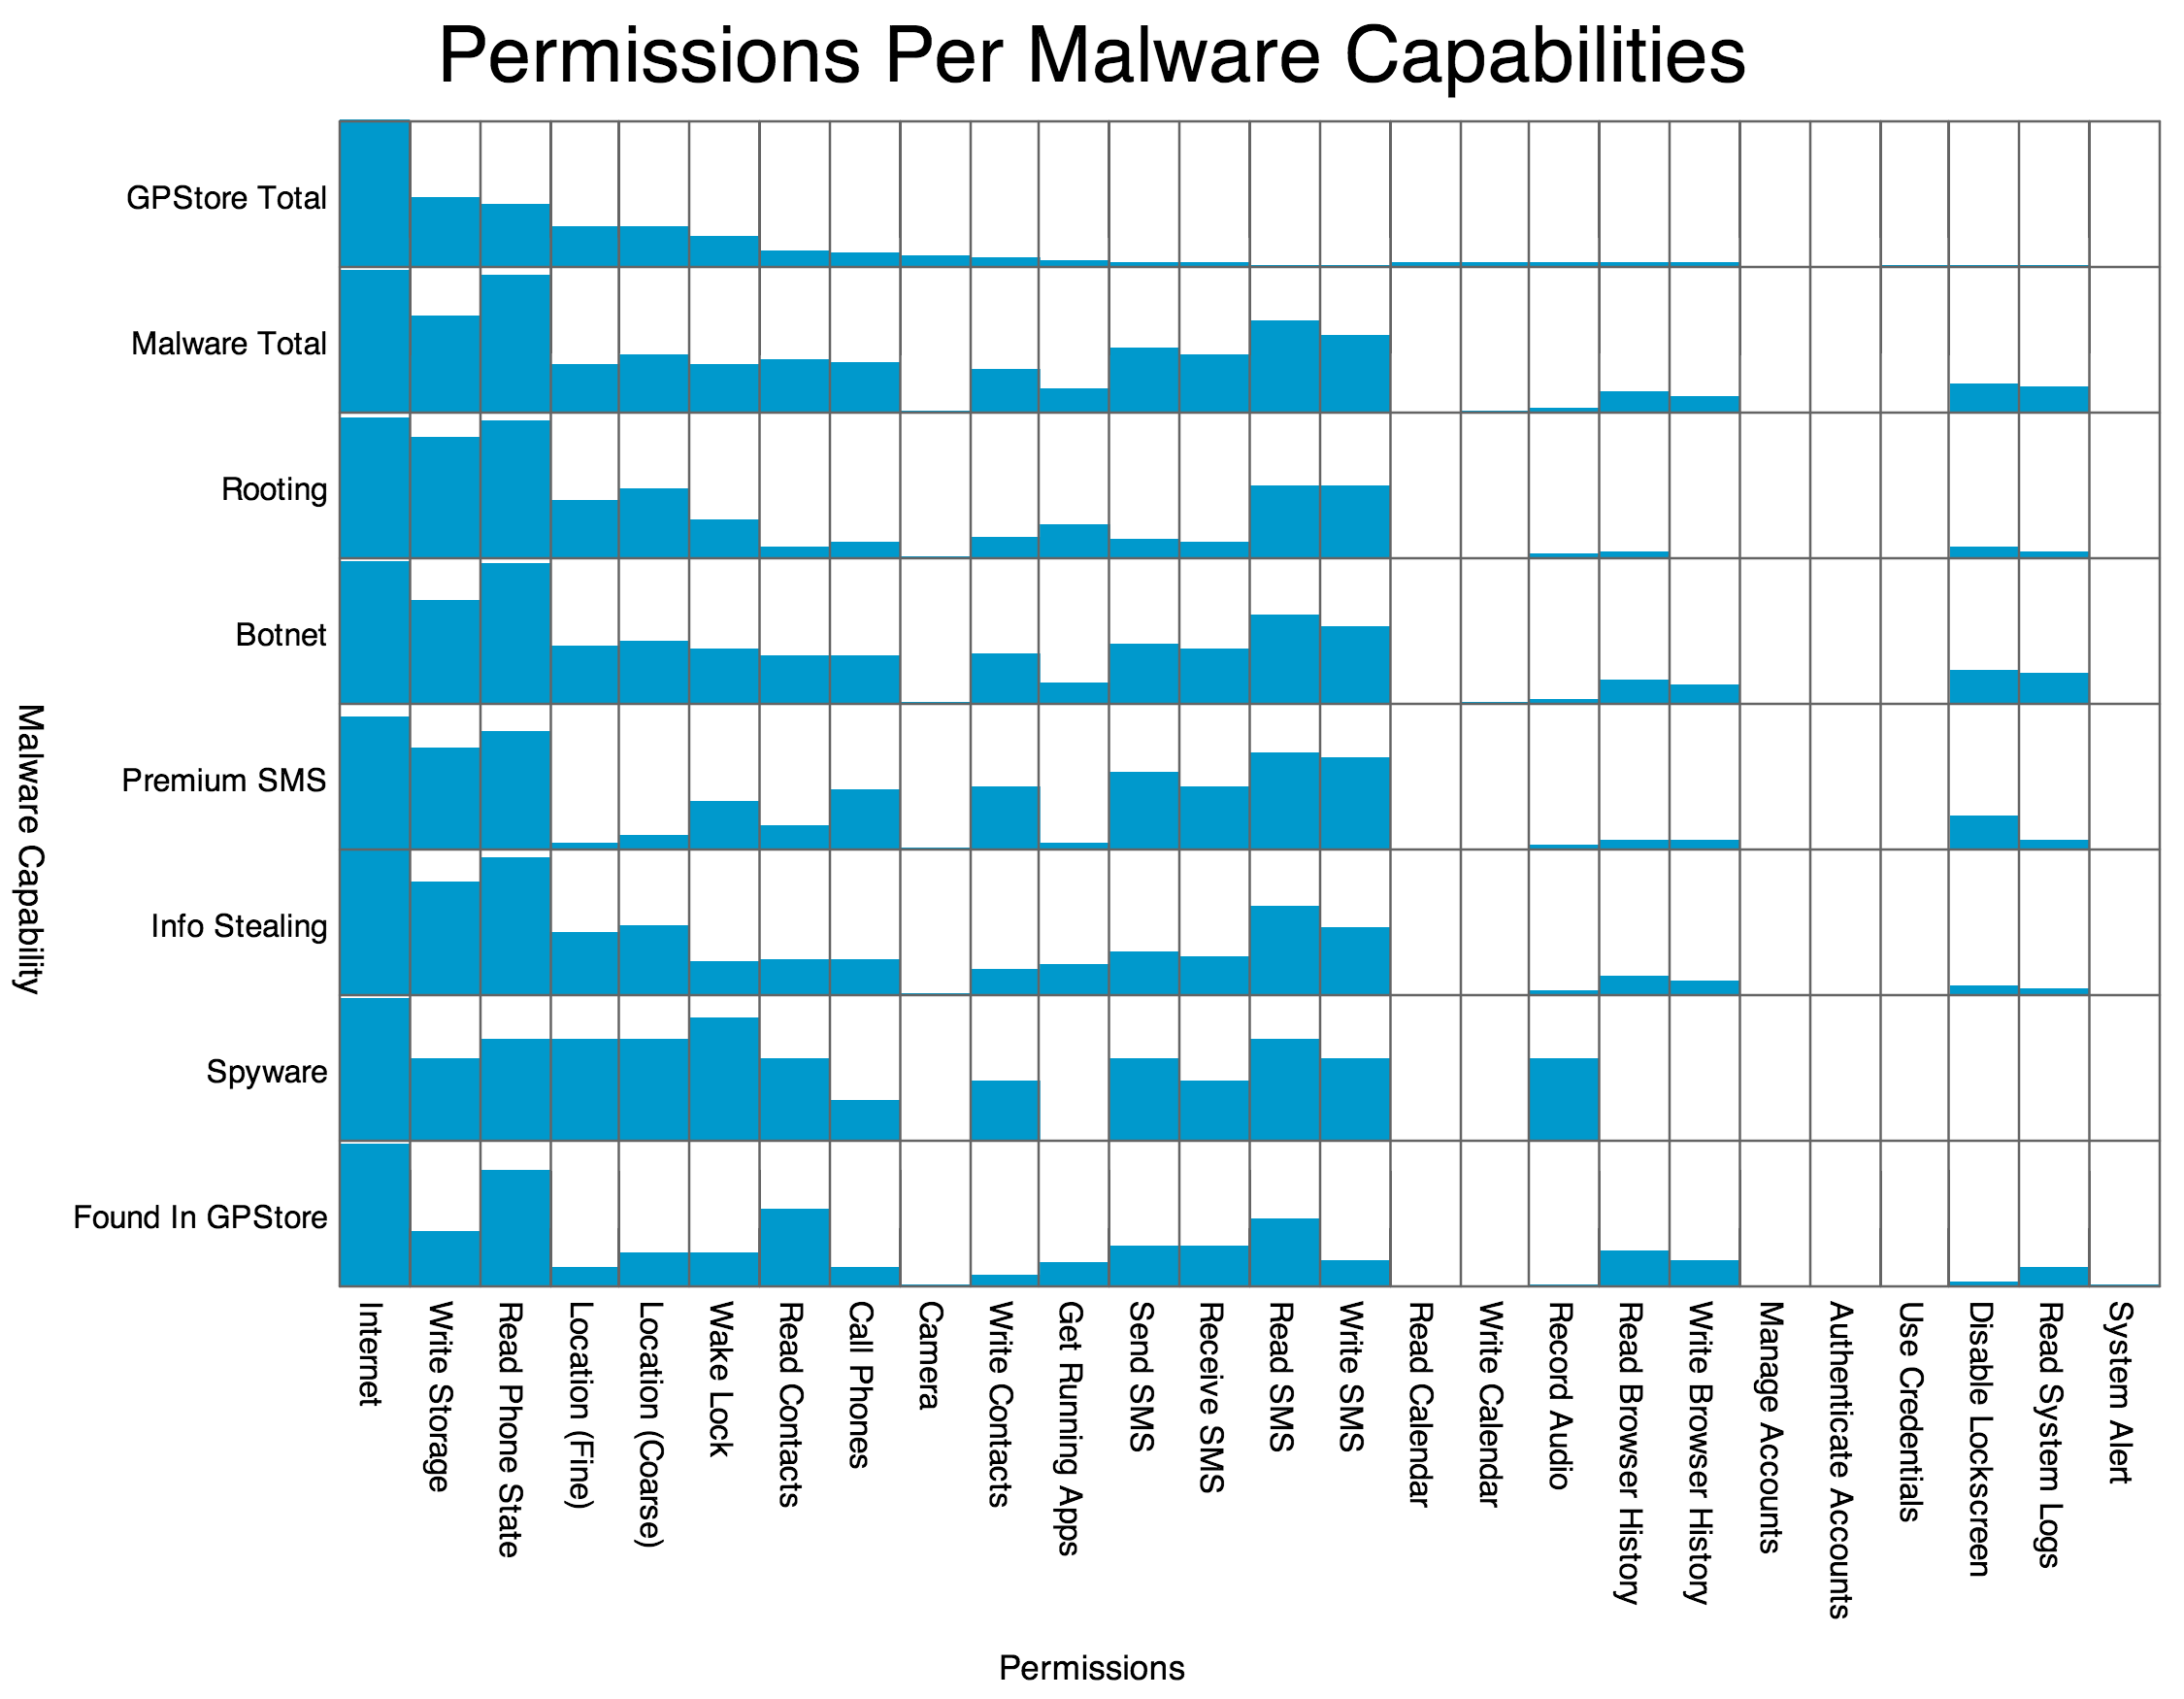
\includegraphics[width=1.0\columnwidth]{figs/MalwareCapabiltiesPermissions}
\caption{Permission Fingerprints of malware with different capabilties, compared to the GPStore total}
\label{fig:malwarefingerprint}
\end{center}
\end{figure}

\subsection{Malware Fingerprints}
The first step in analyzing whether malware Permission Fingerprints are seen as outliers is to obtain permission fingerprints for all apps in the database. After which, we aggregated the fingerprints by classification of capabilities. The result, Figure \ref{fig:malwarefingerprint}, provides a novel look at malware, it's capabilities, and it's permissions relative to the Android market. The differences in Permission Fingerprints, and therefore capabilities of Malware vs the GPStore total become obvious right away. Malware is far more likely to request access to SMS, particularly reading and writing the database, as well as system operations like disabling the lock screen and reading systme logs. 

However, further insight is given when looking at the fingerprints of malware with a specific capability. \textit{Spyware} apps demonstrate this quite clearly: They request access to location, permission to keep the device on at all times, record audio and send SMS messages. These capabilities are what would be expected out of spyware. Likewise, \textit{Premium SMS} apps requested access to Send SMS messages quite often\footnote{The reason this number is not 100\% is because not all variants of a family of malware known to posses a \textit{Premium SMS} exploit may have that capability}. We also observe that \textit{Botnet} malware occasionally accesses system features like disabling the lock screen and reading system logs.

These obversvations are highly valuble, but things break down when we look at the \textit{Info} category. This permission fingerprint, aside from \textit{Read SMS} and \textit{Write SMS}, does not appear significantly different than the GPStore total, especially when considering the Market Category fluctuations observed earlier. 


\section{Popular Apps}
As we have shown, all categories of malware but Info Stealing show profound differences in permission fingerprints: they are far more likely to access unusual permissions than normal Android apps. However, Info stealing apps did not show such anomalies, making them far easier to hide inside of benign apps - a technique malware writers already use\citep{avastfakeapps}. Thus, if more popular apps have more access to PII, this vector poses a serious threat.

For starters, we note that the metadata in \temp{AndroidMarketDB} doesn't give precise download measurements, but rather broad ranges. We plot these in Table \ref{tab:downloadstats}, noting the number of apps in each download range, and it's total percent of all downloads in the market. The top percentile, only 9 apps, accounts for an estimated\footnote{The formula for estimated total downloads was taking the average of the download range, and multiplying it by the number of apps} 11\% of all downloads, and apps over 1 million downloads - only 2250 apps in total - account for an estimated 70\% of all downloads in the entire Google Play Store.

\begin{table*}[t]
\begin{small}
\begin{tabular}{r|llll}
Download Range & Number of Apps & Estimated Total Downloads & Percent of All Downloads & Aggregate Percentage \\
\hline

\textit{100M-500M} & 9 & 2.7B & 11.78\% & 11.78\% \\
\textit{50M-100M} & 12 & 900.0M & 3.93\% & 15.71\% \\
\textit{10M-50M} & 165 & 4.95B & 21.6\% & 37.31\% \\
\textit{5M-10M} & 279 & 2.09B & 9.13\% & 46.44\% \\
\textit{1M-5M} & 1785 & 5.36B & 23.36\% & 69.8\% \\
\textit{500K-1M} & 2010 & 1.51B & 6.58\% & 76.38\% \\
\textit{100K-500K} & 10483 & 3.14B & 13.72\% & 90.1\% \\
\textit{50K-100K} & 9363 & 702.23M & 3.06\% & 93.16\% \\
\textit{10K-50K} & 37925 & 1.14B & 4.96\% & 98.13\% \\
\textit{5K-10K} & 24872 & 186.54M & 0.81\% & 98.94\% \\
\textit{1K-5K} & 66587 & 199.76M & 0.87\% & 99.81\% \\
\textit{500-1K} & 28676 & 21.51M & 0.09\% & 99.91\% \\
\textit{100-500} & 59616 & 17.88M & 0.08\% & 99.98\% \\
\textit{50-100} & 23394 & 1.75M & 0.01\% & 99.99\% \\
\textit{10-50} & 53343 & 1.6M & 0.01\% & 100.0\% \\
\textit{5-10} & 13720 & 96.04K & 0.0\% & 100.0\% \\
\textit{1-5} & 30541 & 91.62K & 0.0\% & 100.0\% \\
\textit{0-0} & 7694 & 0.0 & 0.0\% & 100.0\% \\

\end{tabular}
\end{small}
%\vspace{-0.2in}
\caption{App download statistics from \temp{AndroidMarketDB}}
\label{tab:downloadstats}
%\vspace{-0.1in}
\end{table*}

%\subsection{Top 9 Apps}
%The top 9 apps (in no particular order), are \textit{Facebook}, \textit{GMail}, \textit{Google Maps}, \textit{Google Street View}, \textit{Google Search}, \textit{Google Voice Search}, \textit{Youtube} and \textit{Adobe Flash Player}. It's intriguing yet understandable to see so many Google apps in the top spots, but this is understandable given the fact that these apps have been in the market since very early on.

%The permissions these apps request is atypical of most apps in the GPStore. \textit{Adobe Flash Player} requests no permissions at all, but this is due to it's role as a browser plugin, and is an outlier in this. 

%\subsection{Apps over 1 Million Downloads}
%\temp{Show the same permission histogram as before, but each row is a different download range}

%Discuss it.
Figure \ref{fig:topappsfingerprint} shows the permission fingerprints of the top download categories on the Google Play Store. The apps in the lower ranges, from 10K-50K, show a fingerprint very similar to the overall plot. However, as the install counts rise, several very key permissions rise as well. \textit{Get Running Apps}, \textit{Camera}, \textit{Record Audio}, \textit{Read Contacts}, and \textit{Wake Lock} all spike in popularity, the more installs the app has. These permissions are especially sensitive PII related permissions. Towards the very top, even more permissions become used, \textit{Read and Write SMS} and \textit{Read Browser History}, which are also extremely common malware permissions. Overall, aside from \textit{Read and Write SMS}, the \textit{Info Stealing} malware described above has a surprisingly similar permission fingerprint.

\begin{figure}[h]
\begin{center}
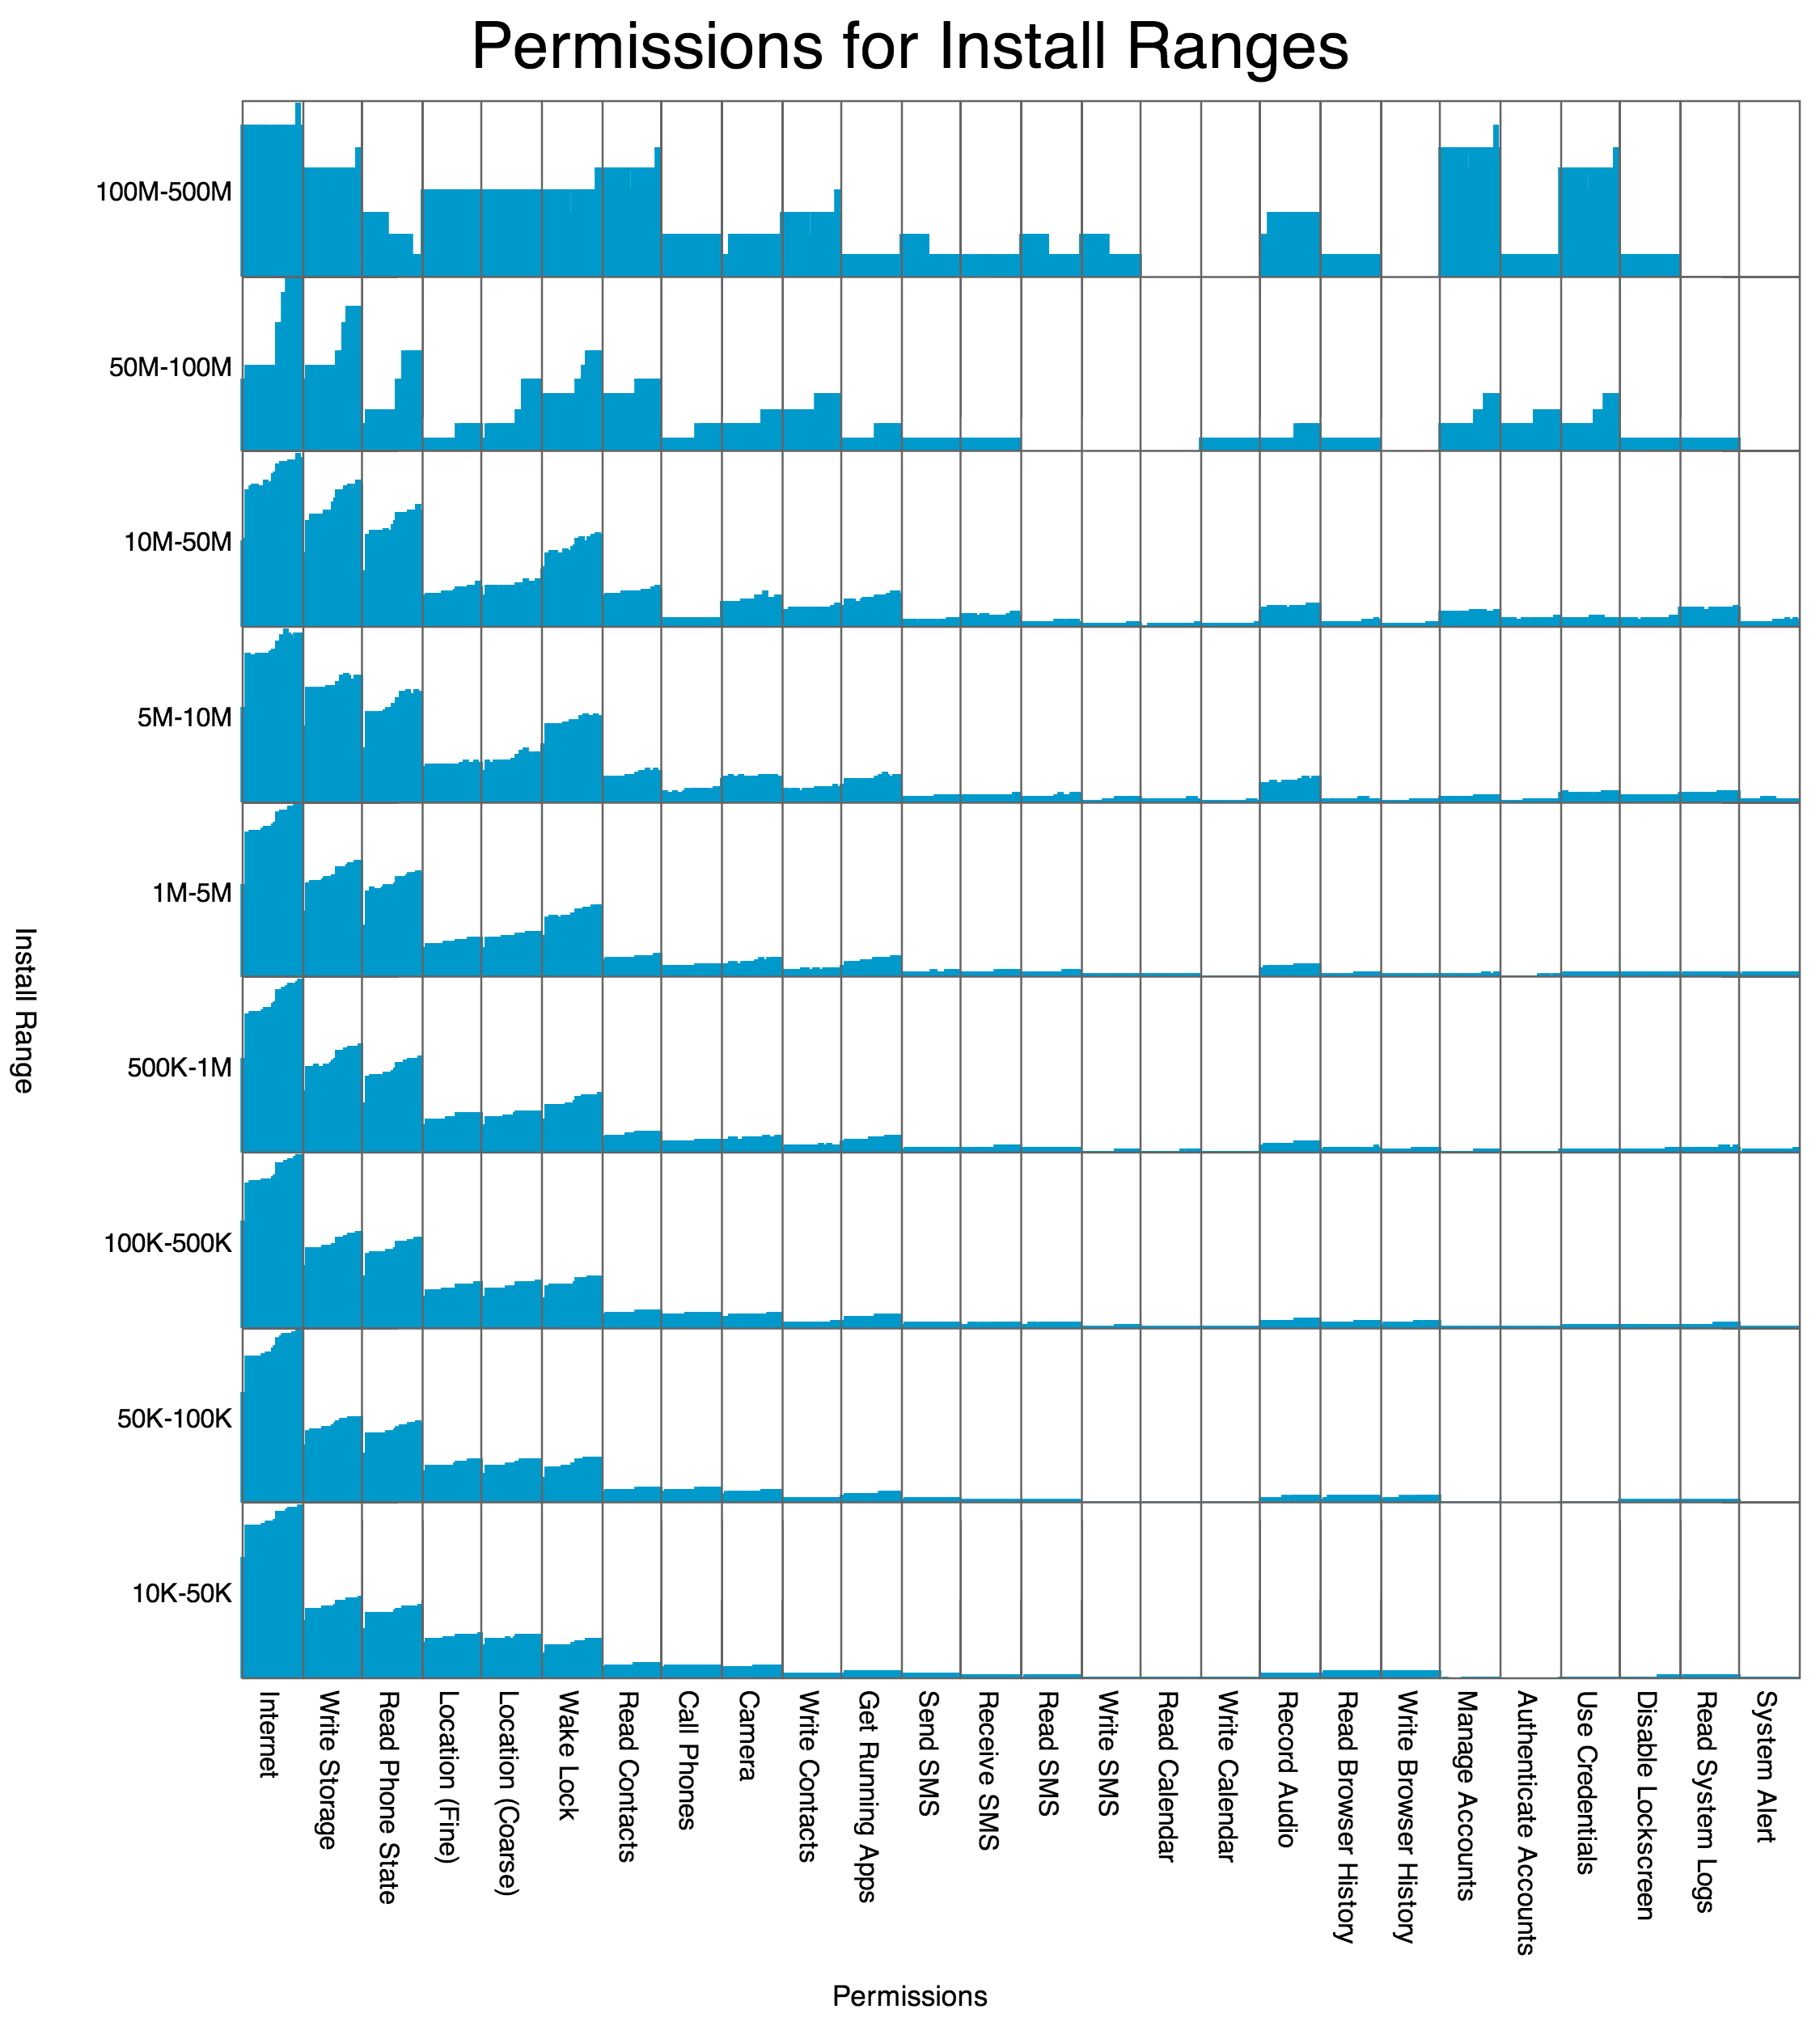
\includegraphics[width=1.0\columnwidth]{figs/PermissionsforInstallRanges}
\caption{Permission Fingerprints of apps with different ranges of install counts}
\label{fig:topappsfingerprint}
\end{center}
\end{figure}



\section{Market Summary}
We have demonstrated several key points in this analysis. First, we demonstrated that Permission Fingerprints, and their aggregate histograms, often correlate with their expected behavior, but found key instances where these did not, especially with respect to PII. We then demonstrated that different classes of malware have permission fingerprints that correlate strongly with their expected behavior, but vary heavily from the rest of the GPStore. However, we noted that \textit{SMS} malware only needed one key permission to operate - one that was ultimately not terribly uncommon in many categories, and info-stealing apps had a permission fingerprint that does not ultimately stick out in the GPStore as a whole. When analyzing the top apps, we found many opportunities for info-stealing malware to imitate their permission fingerprints.

\section{Shortcomings of Permissions on Android}
We have established the limits of Permission Fingerprints: Whereas they list capabilities, they are broad, and do not offer the insight necessary to identify malicious behavior. We have demonstrated that malicious behavior and acceptable behavior can come from the same Permissions. This is ultimately due to two main issues, Permissions do not address the context of use, nor what is done with the data after granting it. These two ideas, context and use, are some defining aspects of the User-App Agreement.